\documentclass[11pt, xcolor=dvipsnames, aspectratio=43]{beamer}
\usetheme{CambridgeUS}
\useoutertheme{infolines}
%\usecolortheme{beaver}
\usepackage[utf8]{inputenc}
\usepackage[english]{babel}
\usepackage{amsmath}
\usepackage{amsfonts}
\usepackage{amssymb}
\usepackage{graphicx}
\usepackage{physics}
\usepackage{hyperref}
\usepackage{siunitx}
\usepackage{booktabs}
\usepackage{makecell}
\usepackage{mhchem}
\usepackage{subcaption}
\usepackage{appendixnumberbeamer}

\newcommand{\tabitem}{~~\llap{\textbullet}~~}

\newcommand{\oper}[1]{\hat{#1}}
\renewcommand{\vec}[1]{\mathbf{\boldsymbol{#1}}}
\newcommand{\vers}[1]{\vec{\hat{#1}}}
\newcommand{\adjoint}[1]{#1^\dagger}
\newcommand{\adjop}[1]{\adjoint{\oper{#1}}}
\newcommand{\sche}{Schr\"{o}dinger equation*\xspace}
\newcommand{\oh}{\frac{1}{2}}
\newcommand{\rr}[1]{#1(\vec{r})}
\newcommand{\dr}{\differential \vec{r}}
\newcommand{\rrp}[1]{#1(\vec{r}')}
\newcommand{\sches}{Schr\"{o}dinger equation*s\xspace}

\DeclareSIUnit\angstrom{\protect \text {Å}}
\DeclareSIUnit{\bohr}{\mu_B}


\useinnertheme{circles}
\setbeamertemplate{caption}[numbered]

\definecolor{UBCblue}{rgb}{0.7, 0, 0} % UBC Blue (primary)
\usecolortheme[named=UBCblue]{structure}

\setbeamercovered{invisible}


\newcommand{\bs}[1]{\boldsymbol{#1}}

\title{Analytical and numerical study of polarons}
\subtitle{A DFT calculation of a small polaron in rutile $\ce{TiO_2}$}
\author[Nicolò Montalti]{Nicolò Montalti \\[3mm]\footnotesize{Relatore: Prof. Cesare Franchini \\ Correlatore: Lorenzo Varrassi}}
\date[22/07/2022]{22 Luglio 2022}
%\setbeamercovered{invisible} 
%\setbeamertemplate{navigation symbols}{} 
%\logo{} 
\institute[University of Bologna]{Laurea in Fisica\\Università di Bologna} 

\begin{document}

\begin{frame}
    \maketitle
\end{frame}

\begin{frame}
    \frametitle{Overview}
    \tableofcontents
\end{frame}

\section{Introduction}

\subsection{Intuitive notion of a Polaron}
\begin{frame}{Intuitive notion of a polaron}
    \begin{figure}
        \centering
        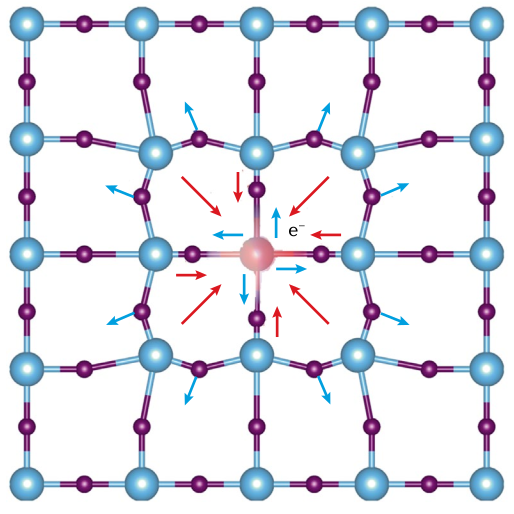
\includegraphics[height=0.7\textheight]{figures/polaron_lattice.png}
        \caption{Figure from Franchini et al. ‘Polarons in materials’, Nature Reviews Materials, Jul. 2021, doi: 10.1038/s41578-021-00289-w.
        }
    \end{figure}
\end{frame}

\subsection{Polarons properties}
\begin{frame}{Band structure and DOS}
    \begin{figure}
        \centering
        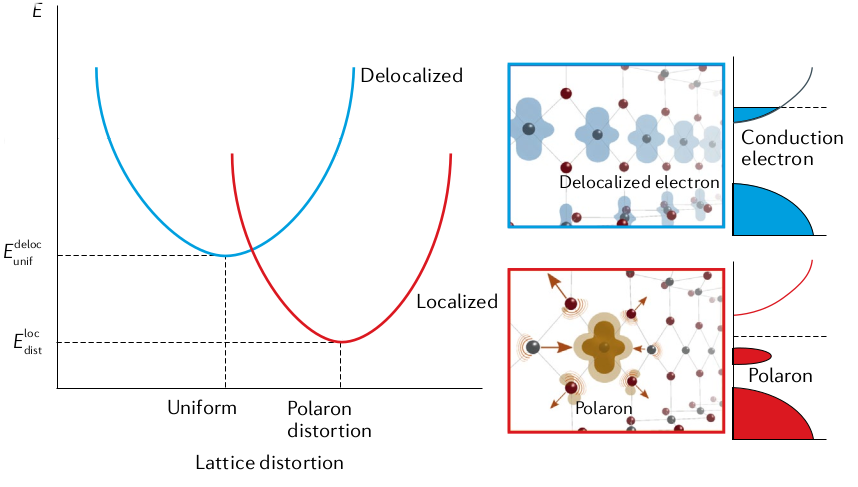
\includegraphics[height=0.7\textheight]{figures/polaron_bands.png}
        \caption{Figures from Franchini et al. ‘Polarons in materials’, Nature Reviews Materials, Jul. 2021, doi: 10.1038/s41578-021-00289-w.
        }
    \end{figure}
\end{frame}


%\begin{frame}{Polarons: a historical overview}
%    \begin{itemize}
%        \item<1-> L. Landau: \emph{Electron Motion in Crystal Lattice} (1933)
%        \item<2-> S. Pekar:
%            \begin{itemize}
%                \item[--]<2-> \emph{Local Quantum States of Electrons in an Ideal Ion Crystal} (1946)
%                \item[--]<2-> \emph{Theory of Colored Crystals} (1947)
%            \end{itemize}
%        \item<3-> L. Landau and S. Pekar: \emph{Effective Mass of a Polaron} (1948)
%        \item<4-> H. Fröhlich et al: \emph{Properties of Slow Electrons in Polar Materials} (1950)
%        \item<5-> T. Holstein: \emph{Studies of Polaron Motion} (1959)
%    \end{itemize}
%\end{frame}

\section{Small and Large Polarons}
%\subsection{Review of Condensed Matter Physics}
%\begin{frame}{Brief review of Condensed Matter Physics}
%    \begin{itemize}
%        \item<1-> Total Hamiltonian
%            \begin{equation*}
%                \oper{H} = \oper{H}_\text{el} + \oper{H}_\text{ph} + \oper{H}_\text{el-ph}
%            \end{equation*}
%        \item<2-> Electrons
%            \begin{equation*}\label{eq:electron_hamiltonian}
%                \oper{H}_\text{el} = \sum_{n\vec{k}} \epsilon_{n\vec{k}} \adjop{c}_{n\vec{k}}\oper{c}_{n\vec{k}}
%            \end{equation*}
%
%        \item<3-> Phonons
%            \begin{equation*} \label{eq:phonon_hamiltonian}
%                \oper{H}_\text{ph} = \sum_{\lambda \vec{q}} \hslash \omega_{\lambda\vec{q}} \left( \adjop{b}_{\lambda \vec{q}} \oper{b}_{\lambda \vec{q}} + \frac{1}{2} \right)
%            \end{equation*}
%        \item<4-> Electron-phonon interaction
%            \begin{equation*} \label{eq:general_electron_phonon_hamiltonian}
%                \oper{H}_\text{el-ph}                = \sum_{\vec{k}'\vec{k}} \sum_{\vec{q}\lambda} M_{\vec{k} \rightarrow \vec{k}'}^\lambda(\vec{q}) \adjop{c}_{\vec{k}'}\oper{c}_{\vec{k}} (\oper{b}_{\vec{q}\lambda} + \adjop{b}_{-\vec{q}\lambda})
%            \end{equation*}
%
%    \end{itemize}
%\end{frame}

\begin{frame}{Small and Large Polarons}
    \begin{minipage}{0.49\textwidth}
        \footnotesize
        \begin{equation*}
            \oper{H}_\text{el-ph} = \frac{g}{\sqrt{N}}\sum_{\vec{k}, \vec{q}} \adjop{c}_{\vec{k}+\vec{q}} \oper{c}_\vec{k} (\adjop{b}_{-\vec{q}} + \oper{b}_\vec{q})
        \end{equation*}
    \end{minipage}
    \begin{minipage}{0.49\textwidth}
        \footnotesize
        \begin{equation*}
            \oper{H}_\text{el-ph} = C \sum_{\vec{k},\vec{q}} \left| \vec{q} \right|^{-1}\adjop{c}_{\vec{k}+\vec{q}}\oper{c}_{\vec{k}} (\oper{b}_{\vec{q}} + \adjop{b}_{-\vec{q}})
        \end{equation*}
    \end{minipage}
    \begin{figure}[p]
        \begin{subfigure}[b]{0.42\textwidth}
            \centering
            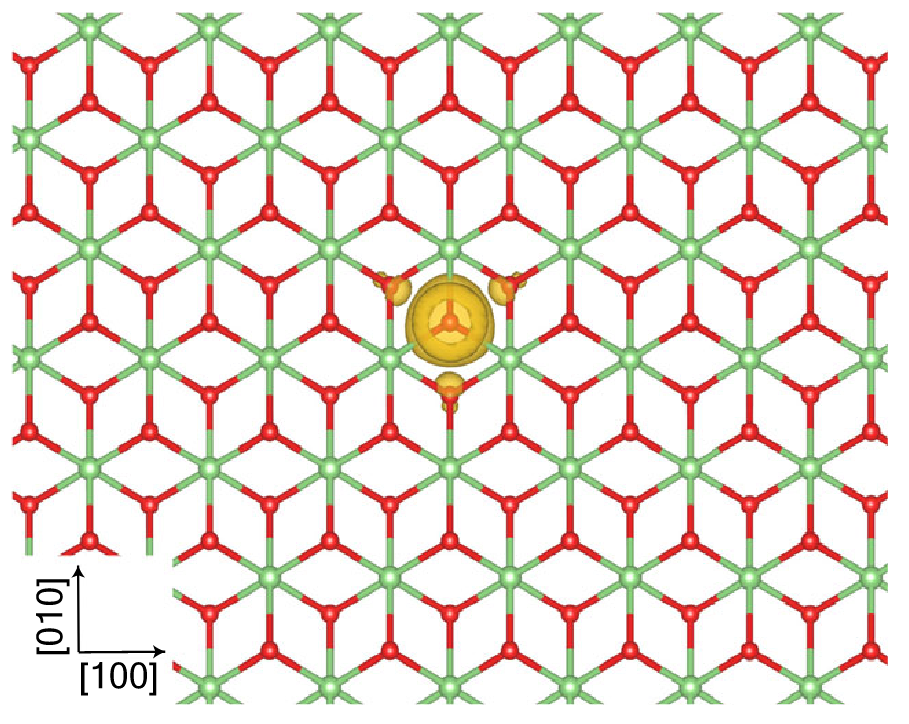
\includegraphics[width=\textwidth]{figures/small.png}
            \caption{Small (Holstein) polaron}
            \label{fig:small}
        \end{subfigure}
        \hfill
        \begin{subfigure}[b]{0.49\textwidth}
            \centering
            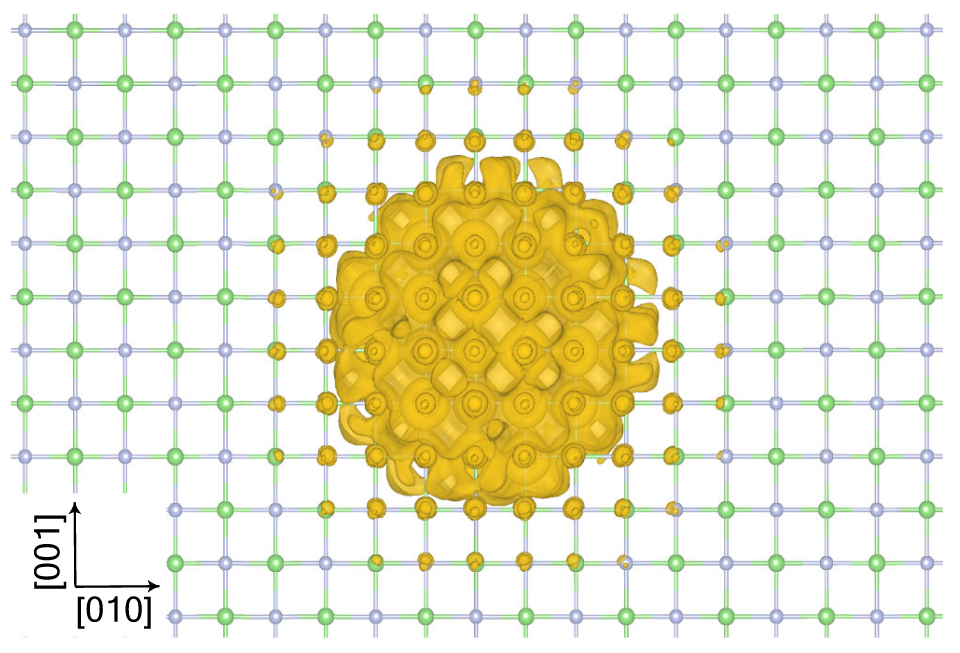
\includegraphics[width=\textwidth]{figures/large.png}
            \caption{Large (Fröhlich) polaron}
            \label{fig:large}
        \end{subfigure}
        \caption{Figures from W. H. Sio et al., ‘Polarons from First Principles, without Supercells’, Jun. 2019, doi: 10.1103/PhysRevLett.122.246403}.
        \label{fig:small_large}
    \end{figure}
\end{frame}

\section{Density Functional Theory}
\begin{frame}{Density Functional Theory}
    Basic assumption: the ground-state energy of the system $E_g$ is a \alert{functional $E_g[\rho]$ of the sole charge density $\rho$}, where
    \begin{equation*}
        \rho(\vec{r}) = \sum_i \bra{\Psi} \delta^3(\vec{r}-\vec{r}_i)\ket{\Psi}
    \end{equation*}
    \pause
    Given the Hamiltonian
    \begin{equation*} \label{eq:hamiltonian_DFT}
        \oper{H} = \sum_i v(\vec{r}_i) + \sum_i \frac{\vec{p}_i^2}{2m} + \oh \sum_{i\neq j} \frac{e^2}{|\vec{r}_i - \vec{r}_j|} = V + T + U
    \end{equation*}
    the charge density is found \alert{minimizing}
    \begin{equation*} \label{eq:ground_functional}
        E_g[\rho] = \bra{\Psi[\rho]} V+T+U \ket{\Psi[\rho]} = \int v(\vec{r}) \rho(\vec{r}) \differential \vec{r} + F[\rho]
    \end{equation*}
\end{frame}

\begin{frame}{Kohn-Sham equations}
    To solve the problem, we consider a \alert{fictitious system of non-interacting particles} with the same density $\rho(\vec{r})$
    \begin{align*}
        U_\text{KS} & = \frac{e^2}{2} \int \frac{\rho(\vec{r})\rho(\vec{r}')}{|\vec{r}-\vec{r}'|}  \dr \dr' \\
        T_\text{KS} & = -\frac{\hslash^2}{2m}\sum_i \int \rr{\phi_i^*} \laplacian \rr{\phi_i} \dr
    \end{align*}
    \pause
    The difference with the real system is encoded in the exchange-correlation energy term \alert{$E_\text{xc}$}
    \begin{equation*}
        F[\rho]      = T_\text{KS}[\rho] + U_\text{KS}[\rho] + E_\text{xc}[\rho]
    \end{equation*}
    %\pause
    %usually parametrized as
    %\begin{equation*}
    %    E_\text{xc}^\text{LDA}  = \int \rr{\rho} \epsilon_\text{xc}(\rho) \dr             \qquad
    %    E_\text{xc}^\text{GGA}  = \int \rr{\rho} \epsilon_\text{xc}(\rho, \grad \rho) \dr
    %\end{equation*}
    which has no exact known expression, and it is therefore parametrized.
\end{frame}

\begin{frame}{Kohn-Sham equations}
    The charge density that minimize the energy of the real system $E_g[\rho]$ is found solving the \alert{Kohn-Sham equations}
    \begin{equation*} \label{eq:kohn_sche}
        \left(-\frac{\hslash^2}{2m} \laplacian + \rr{v} + \rr{v_H} + \rr{v_\text{xc}} \right) \rr{\phi_i} = \epsilon_i \rr{\phi_i}
    \end{equation*}
    where
    \begin{equation*}
        \rr{v_H}          = e^2 \int \frac{\rho'(\vec{r}')}{|\vec{r}-\vec{r}'|} \dr' \qquad \quad
        \rr{v_\text{xc}}  =  \frac{\delta E_\text{xc}}{\delta\rr{\rho'}}
    \end{equation*}
    \begin{equation*} \label{eq:kohn_rho}
        \rr{\rho} = \rr{\rho'} = \sum_i |\rr{\phi_i}|^2
    \end{equation*}
    \pause
    The energy of the real system is given by
    \begin{equation*} \label{eq:ground_functional}
        E_g[\rho]  = \int v(\vec{r}) \rho(\vec{r}) \differential \vec{r} + T_\text{KS}[\rho] + U_\text{KS}[\rho] + E_\text{xc}[\rho]
    \end{equation*}
\end{frame}

\section{Simulation of a small polaron}
\subsection{Employed rocedure}
\begin{frame}{DFT on Rutile TiO2}{}

    \alert{Unit cell} \\
    \begin{minipage}[]{0.49\linewidth}
        \begin{enumerate}
            \item Structure relaxation
            \item Standard DFT calculation
            \item DFT+U calculation with $U = \SI{3.9}{eV}$
        \end{enumerate}
    \end{minipage}
    \begin{minipage}{0.49\linewidth}
        \centering
        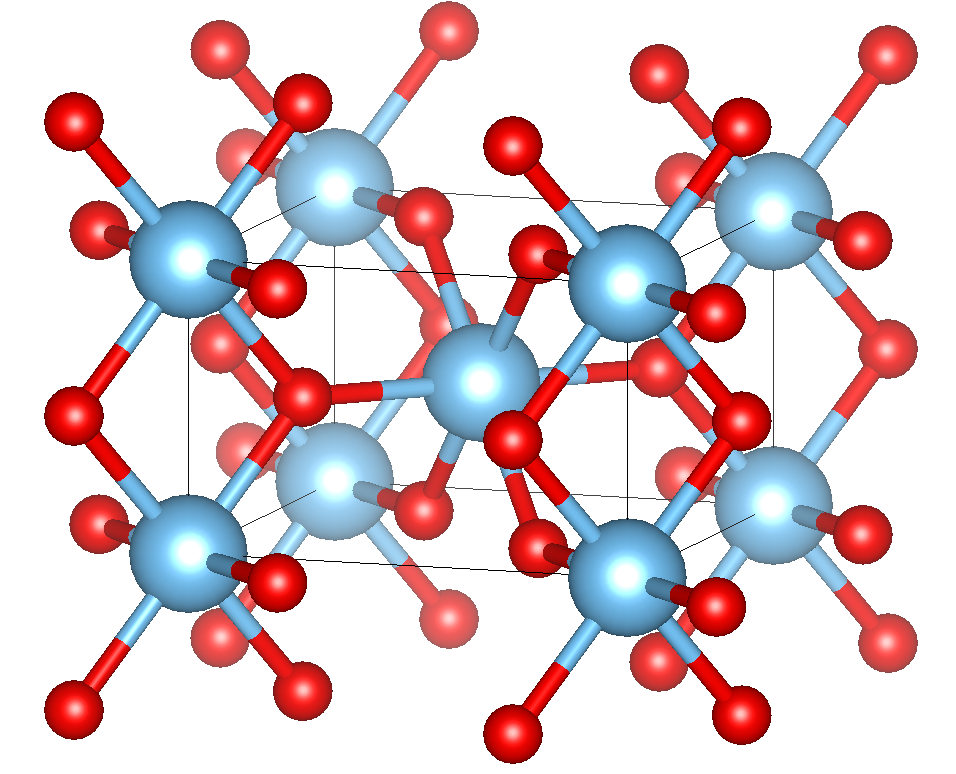
\includegraphics[width=0.65\textwidth]{figures/rutile.png}
    \end{minipage}
    \pause
    \alert{Supercell} \\
    \begin{minipage}[]{0.49\linewidth}
        \begin{enumerate}
            \setcounter{enumi}{3}
            \item DFT calculation with $U = \SI{3.9}{eV}$
            \item Extra electron localization
        \end{enumerate}
    \end{minipage}
    \begin{minipage}{0.49\linewidth}
        \centering
        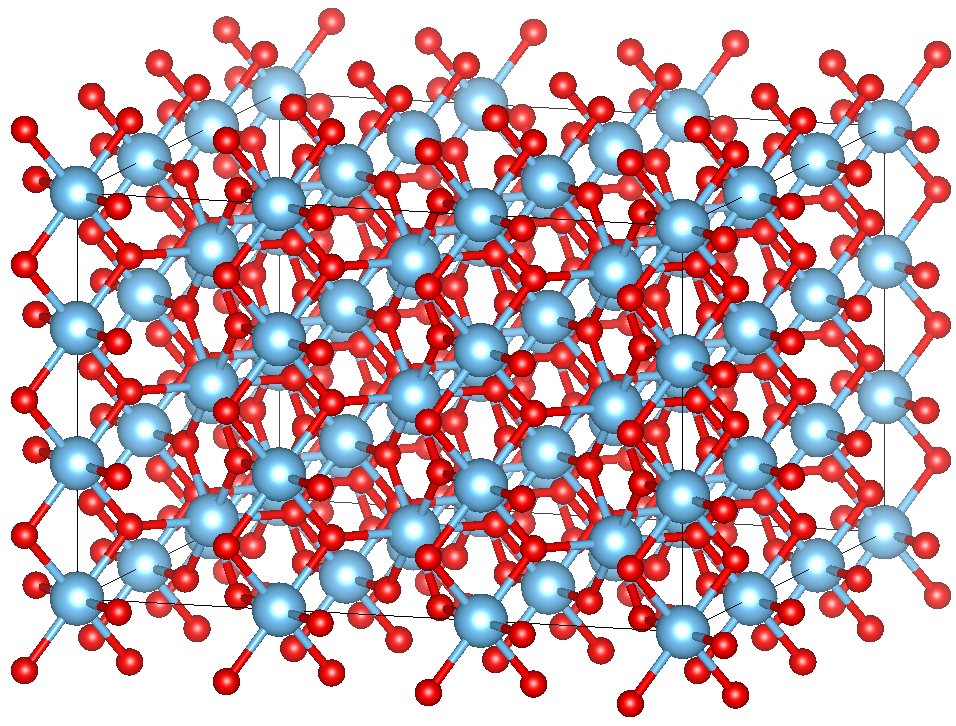
\includegraphics[width=0.65\textwidth]{figures/supercell.png}
    \end{minipage}
\end{frame}

\begin{frame}{Polaron in Rutile TiO2}
    \alert{Electron localization} \\
    \begin{minipage}[]{0.49\linewidth}
        \begin{enumerate}
            \setcounter{enumi}{5}
            \item Vanadium, $U = \SI{9}{eV}$
        \end{enumerate}
    \end{minipage}
    \begin{minipage}{0.49\linewidth}
        \centering
        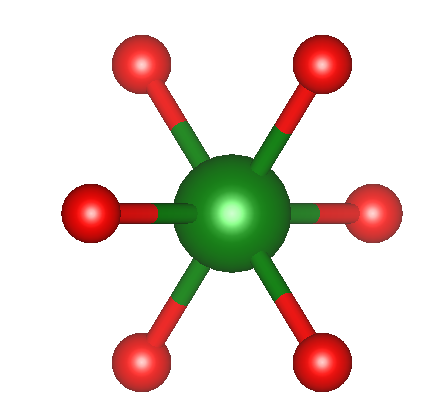
\includegraphics[width=0.5\textwidth]{figures/vanadium.png}
    \end{minipage}
    \pause
    \begin{minipage}[]{0.49\linewidth}
        \begin{enumerate}
            \setcounter{enumi}{6}
            \item Titanium, $U = \SI{9}{eV}$
            \item Titanium, $U = \SI{3.9}{eV}$
        \end{enumerate}
    \end{minipage}
    \begin{minipage}{0.49\linewidth}
        \centering
        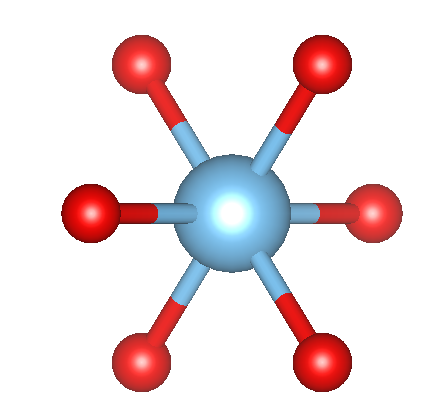
\includegraphics[width=0.5\textwidth]{figures/titanium.png}
    \end{minipage}

\end{frame}

\subsection{Results}

\begin{frame}{Rutile TiO2 band structure}
    \begin{figure}
        \centering
        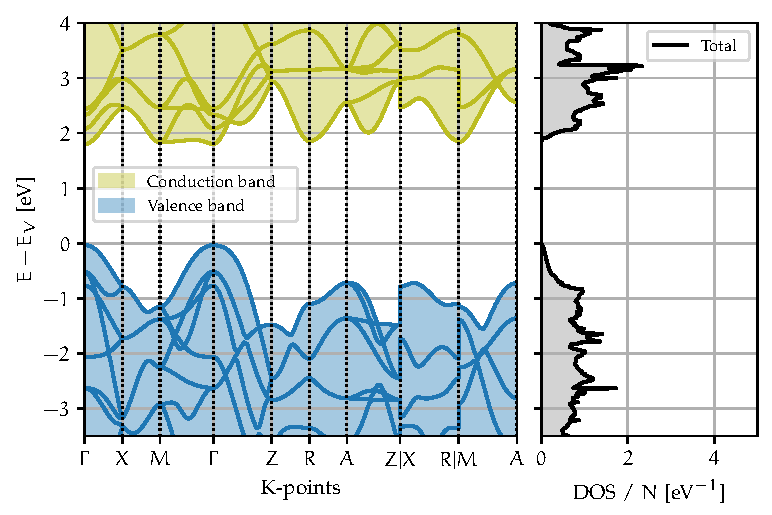
\includegraphics[height=0.7\textheight]{figures/unit.pdf}
        \caption{Band structure and DOS of the rutile unit cell (standard DFT). The direct $\Gamma - \Gamma$ energy gap in is of \SI{1.83}{eV}.}
        \label{fig:bands_unit}
    \end{figure}
\end{frame}

\begin{frame}{Rutile TiO2 band structure (DFT+U)}
    \begin{figure}
        \centering
        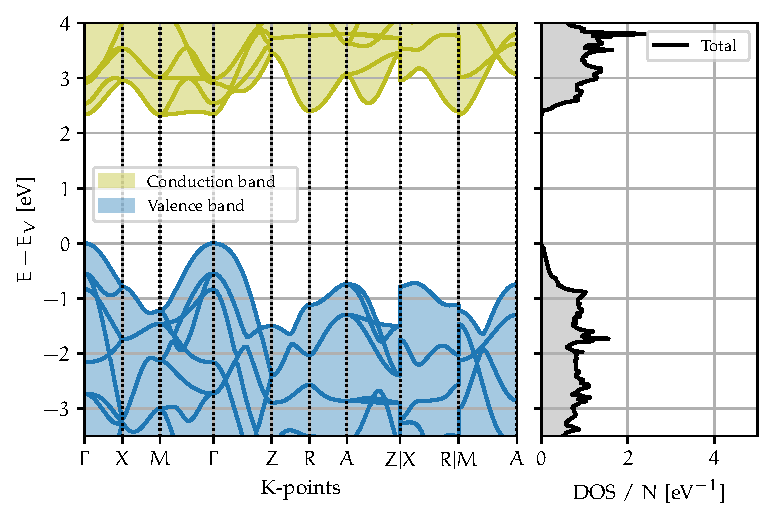
\includegraphics[height=0.7\textheight]{figures/unit+u.pdf}
        \caption{Band structure and DOS of the rutile unit cell (DFT+U, $U=\SI{3.9}{eV}$). The direct $\Gamma - \Gamma$ energy gap in is of \SI{2.33}{eV}.}
        \label{fig:bands_unit}
    \end{figure}
\end{frame}


\begin{frame}{Rutile TiO2 supercell band structure}
    \begin{figure}
        \centering
        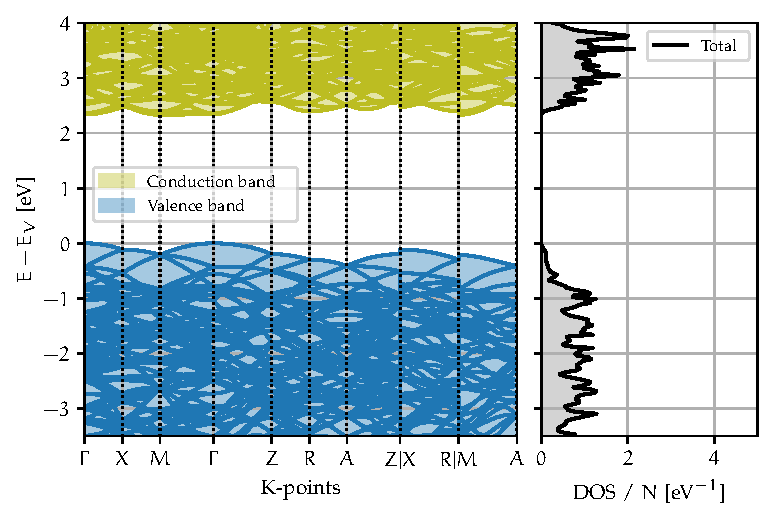
\includegraphics[height=0.7\textheight]{figures/super.pdf}
        \caption{Band structure and DOS of the rutile supercell (DFT+U, $U=\SI{3.9}{eV}$). The direct $\Gamma - \Gamma$ energy gap in is of \SI{2.33}{eV}.}
        \label{fig:bands_unit}
    \end{figure}
\end{frame}


\begin{frame}{Polaron band structure}
    \begin{figure}
        \centering
        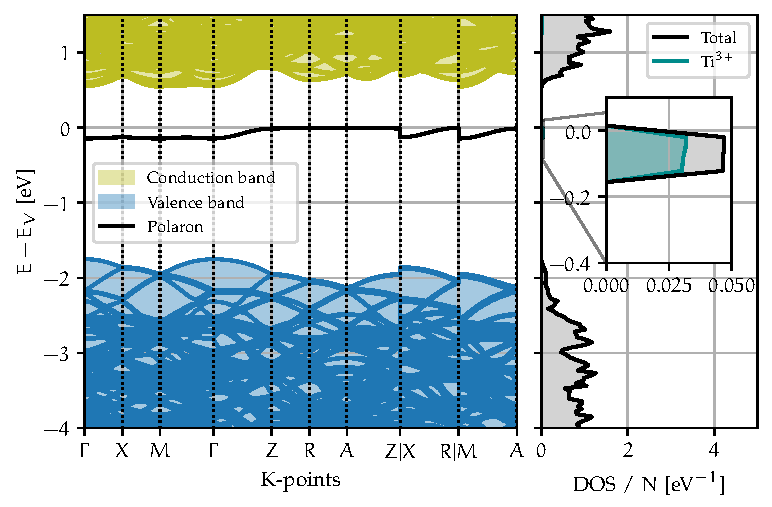
\includegraphics[height=0.7\textheight]{figures/polaron.pdf}
        \caption{Band structure and DOS of the supercell with an extra electron localized on the central atom. An extra state is formed \SI{0.70}{eV} below the conduction band.}
    \end{figure}
\end{frame}


\begin{frame}{Delocalized electron band structure}
    \begin{figure}
        \centering
        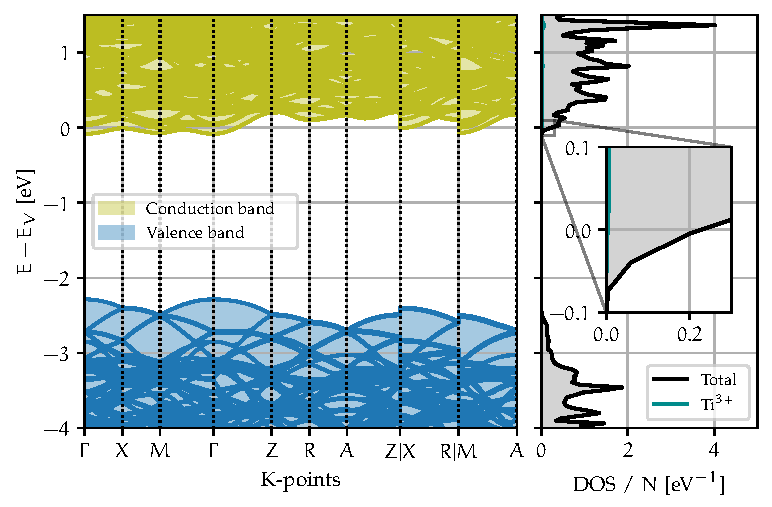
\includegraphics[height=0.7\textheight]{figures/deloc.pdf}
        \caption{Band structure and DOS of the supercell with an extra electron delocalized in the material. The electron enters the conduction band.}
    \end{figure}
\end{frame}

\begin{frame}{Charge isosurface}
    %\centering
    %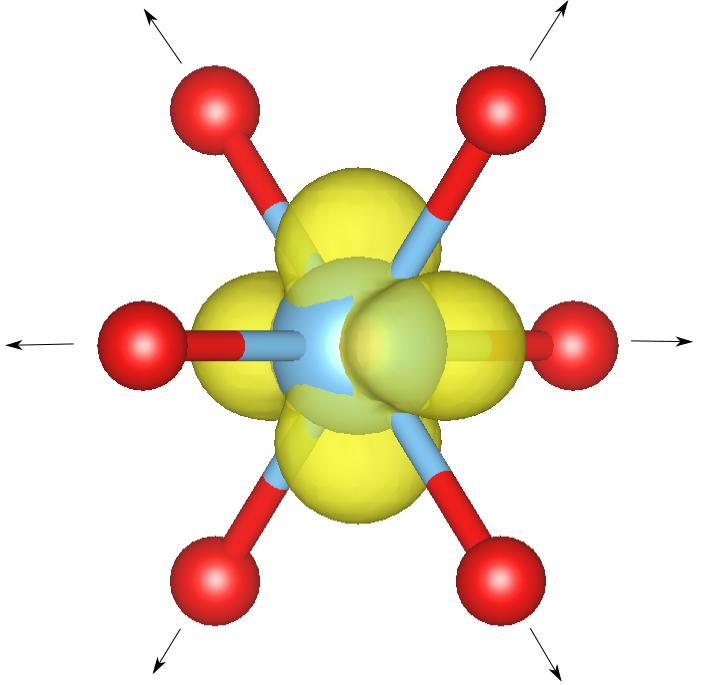
\includegraphics[width=0.45\textwidth]{figures/PARCHG_polaron}
    %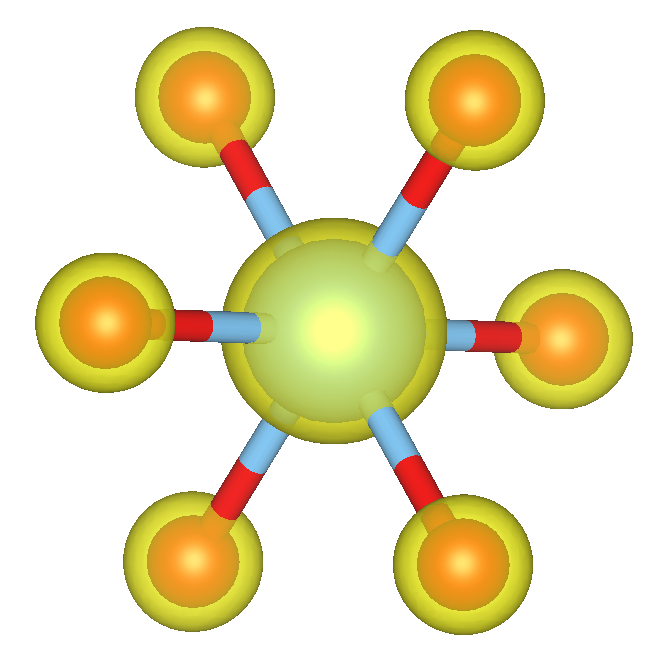
\includegraphics[width=0.45\textwidth]{figures/PARCHG_delocalized.png}
    %
    \begin{figure}[p]
        \centering
        \begin{subfigure}[b]{0.49\textwidth}
            \centering
            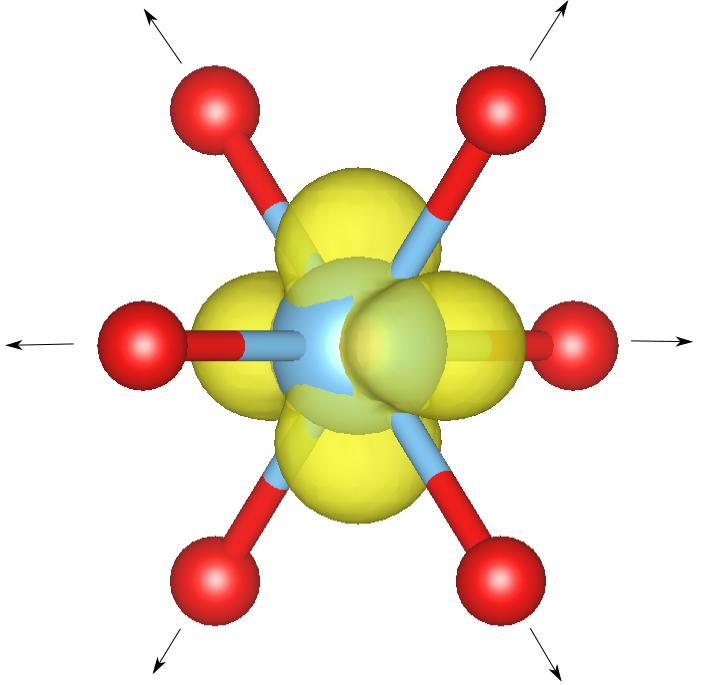
\includegraphics[height=0.53\textheight]{figures/PARCHG_polaron}
            \caption{Electron localized: polaron}
            \label{fig:polaron_iso}
        \end{subfigure}
        \hfill
        \begin{subfigure}[b]{0.49\textwidth}
            \centering
            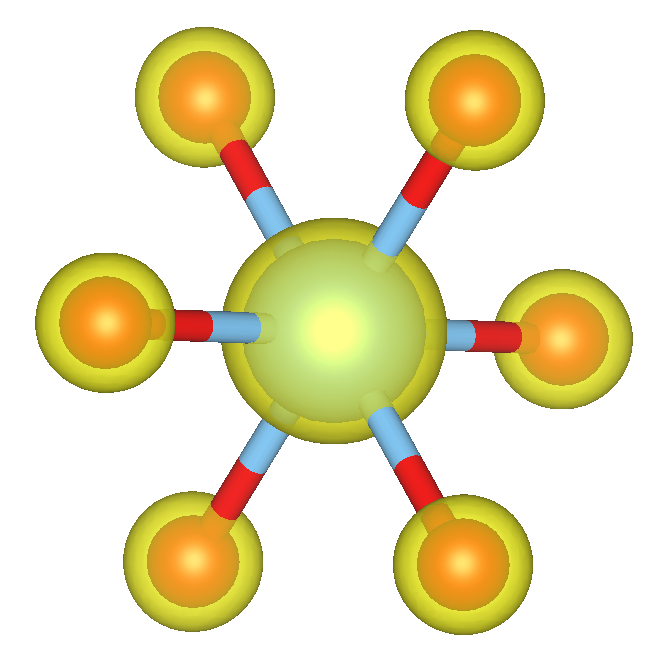
\includegraphics[height=0.53\textheight]{figures/PARCHG_delocalized}
            \caption{Electron delocalized}
            \label{fig:delocalized_iso}
        \end{subfigure}
        \caption{Central atom with the isosurface  (10\%) of the charge density projected on the extra-electron band. In (a) The four oxygen atoms closer to the titanium atom are displaced by \SI{0.085}{\angstrom} outwards, whereas the two further oxygen atoms by \SI{0.023}{\angstrom}.}
        \label{fig:isosurfaces_center}
    \end{figure}
\end{frame}

\section{Conclusions}
\begin{frame}{Take home messages}
    \begin{itemize}
        \item<1-> A Polaron is formed by an electron \alert{distorting} the lattice and creating a \alert{potential well} in which it \alert{localizes}
        \item<2-> An \alert{extra state} is formed below the conduction band, the effective mass is increased
        \item<3-> Small Polarons can be simulated using \alert{DFT} and compared with delocalized electrons
    \end{itemize}
\end{frame}

\section*{Thank you}
\begin{frame}{}
    \centering \huge
    \emph{\alert{Thank you}\\for your attention}
\end{frame}

\appendix
\section*{Appendices}

\begin{frame}{DFT+U}
    \begin{itemize}
        \item<1-> Fundamental problem in DFT: \alert{Hartree} term
            \begin{equation*}
                U_\text{KS} = \frac{e^2}{2} \int \frac{\rho'(\vec{r})\rho'(\vec{r}')}{|\vec{r}-\vec{r}'|} \dr \dr'
            \end{equation*}
        \item<2-> Exchange-correlation energy cannot counterbalance it
            \begin{equation*}
                E_\text{xc}^\text{GGA}  = \int \rr{\rho} \epsilon_\text{xc}(\rho, \grad \rho) \dr
            \end{equation*}
        \item<3-> Correction with an \alert{Hubbard}-like Hamiltonian
            \begin{equation*}
                \oper{H}_\text{Hub} = -t \sum_{\langle i,j \rangle} \adjop{c}_{j,\sigma}\oper{c}_{j,\sigma} + U \sum_i \oper{N}_{i\uparrow} \oper{N}_{i\downarrow}
            \end{equation*}
        \item<4-> \alert{Duradev}: dependency only on $U-t$. The greater the value assigned to $U$ is, the more the states are \alert{localized} and the more the gap broadens.
    \end{itemize}
\end{frame}

\begin{frame}{Small and Large Polarons properties}
    \resizebox{\textwidth}{!}{%
        \begin{tabular}{ll}
            \toprule
            \multicolumn{1}{c}{
            \alert{Small} (Holstein) polarons                  } & \multicolumn{1}{c}{ \alert{Large} (Fröhlich) polarons                 } \\
            \midrule
            \multicolumn{1}{c}{
            $\oper{H}_\text{el-ph} = \frac{g}{\sqrt{N}}\sum_{\vec{k}, \vec{q}} \adjop{c}_{\vec{k}+\vec{q}} \oper{c}_\vec{k} (\adjop{b}_{-\vec{q}} + \oper{b}_\vec{q})$
            }                                                    & \multicolumn{1}{c}{
            $\oper{H}_\text{el-ph} = C \sum_{\vec{k},\vec{q}} \left| \vec{q} \right|^{-1}\adjop{c}_{\vec{k}+\vec{q}}\oper{c}_{\vec{k}} (\oper{b}_{\vec{q}} + \adjop{b}_{-\vec{q}})$          }
            \\
            \midrule
            \tabitem Short-range electron-phonon interaction     & \tabitem Long-range electron-phonon interaction                         \\
            \tabitem Polaron radius $\approx$ lattice parameter  & \tabitem Polaron radius $\gg$ lattice parameter                         \\
            \tabitem Narrow mid-gap electronic state             & \tabitem Shallow mid-gap electronic state                               \\
            $\qquad (\approx \SI{1}{eV}$ below $E_F$)            & $\qquad (\approx \SI{10}{meV}$ below $E_F$)                             \\

            \tabitem Incoherent motion (phonon assisted)         & \tabitem Coherent motion                                                \\
            \tabitem Thermally activated hopping mobility        & \tabitem Free carrier mobility                                          \\
            $\qquad \ll \SI{1}{cm^2 V^{-1} s^{-1}}$              & $\qquad \gg \SI{1}{cm^2 V^{-1} s^{-1}}$                                 \\
            \tabitem Mobility increasing with temperature        & \tabitem Mobility decreasing with temperature                           \\
            \bottomrule
        \end{tabular}
    }
\end{frame}

\begin{frame}{Fröhlich Hamiltonian}
    \begin{multline*} \label{eq:frohlich_hamiltonian}
        H_\text{Fröhlich} = \sum_{\vec{k}} \frac{\hslash^2\vec{k}^2}{2m}
        + \sum_{\vec{q}} \hslash \omega_\text{LO} \left( \adjop{b}_{ \vec{q}} \oper{b}_{ \vec{q}} + \frac{1}{2} \right)
        \\ + \sum_{\vec{k}\vec{q}} \frac{\hslash \omega_\text{LO}}{|\vec{q}|} \left(\frac{\hslash}{2m\omega_\text{LO}}\right)^{1/4} \left(\frac{4\pi\alpha}{\Omega}\right)^{1/2} \adjop{c}_{\vec{k}}\oper{c}_{\vec{k}-\vec{q}} (\oper{b}_{\vec{q}} + \adjop{b}_{-\vec{q}})
    \end{multline*}
    \begin{itemize}
        \item Weak-coupling limit
              \begin{equation*}
                  E_\vec{k}                           = -\alpha \hslash \omega_\text{LO} + \left(1 - \frac{\alpha}{6}\right)\frac{\hslash^2}{2m}k^2
                  %\end{equation*}
                  %\begin{equation*}
                  \qquad
                  \langle \oper{N}_\text{ph} \rangle  = \sum_\vec{q} \bra{\psi} \adjop{b}_\vec{q} \oper{b}_\vec{q} \ket{\psi} = \frac{\alpha}{2}
              \end{equation*}
        \item Strong-coupling limit
              \begin{equation*}
                  E_\text{var} = -\frac{\alpha^2}{3\pi} \hslash\omega_\text{LO}
              \end{equation*}
    \end{itemize}
\end{frame}

\begin{frame}{Holstein Hamiltonian}
    \begin{multline*}
        \oper{H}_\text{Holstein} = \sum_{\vec{k}} \epsilon_{\vec{k}}^\text{tb} \adjop{c}_{\vec{k}}\oper{c}_{\vec{k}} + \hslash \omega_0\sum_{\vec{q}}  \left( \adjop{b}_{\vec{q}} \oper{b}_{\vec{q}} + \frac{1}{2} \right) + \\
        \frac{g}{\sqrt{N}}\sum_{\vec{k}, \vec{q}} \adjop{c}_{\vec{k}+\vec{q}} \oper{c}_\vec{k} (\adjop{b}_{-\vec{q}} + \oper{b}_\vec{q})
    \end{multline*}
    \begin{itemize}
        \item Weak-coupling limit
              \begin{equation*}
                  E_k = -2t\cos(k)  - \frac{1}{2\pi}\int \differential q \frac{\alpha \hslash \omega_0 t}{2t\cos(k) +2t\cos(k-q) - \hslash \omega_0 }
              \end{equation*}
    \end{itemize}

\end{frame}



\end{document}
